\section{Numerical experiments on stalling resolution} \label{sec:dykstra_numerical_experiments}

We demonstrate the fundamental efficacy of the fast-forward modification through two different example. The first, discussed in Section~\ref{subsec:line_box_example}, comprises the foundational motivating experiment from~\cite{DYKSTRASTALLING}. The second acts as a numerical benchmark between the ``vanilla'' implementation and our implementation (Algorithm~\ref{alg:fastforward}) on randomly generated constraints, and is discussed in section~\ref{subsec:randomly_generated_constraints}. The results of our experiments can be reproduced from the first of two repositories that accompany this thesis~\cite{DykstraProjectRepo, DykstraOptimalTransportRepo}, which can be found at:

\begin{center}
    \href{https://github.com/ClouD-161803/Senior-Thesis-4YPe.git}{ClouD-161803/Dykstra-Project.git}.
\end{center}

\subsection{The line-box example} \label{subsec:line_box_example}

 The selected example evaluates the Euclidean projection of an initial point $w^\circ$ onto the intersection of a box and a single line in $\mathbb{R}^2$ ($d=2$). The box is centred at the origin and is defined by the bounds $ [-1, 1] \times [-1, 1]$, while the line passes through the spatial coordinates $(0,1)$ and $(2, 0)$. This specific pathological configuration was first described in detail by Bauschke et al.~\cite{DYKSTRASTALLING}, which motivates our research on stalling for Dykstra's algorithm. 

The initial point was explicitly set to $w^\circ = (-4, 1.4)$ to artificially induce a prolonged stalling period. To serve as an absolute benchmark for error calculations, the ground-truth optimal solution $w^\star$ was independently computed using the heavy interior-point CQP solver \texttt{quadprog}~\cite{goldfarb1983quadprog, turlach2019quadprog}. During the execution of both projection algorithms, individual half-space activity was monitored by verifying the condition defined in~\eqref{eq:halfspaces_i} for each set at every iteration. The overall convergence behaviour was tracked via the squared $\ell_2$-norm of the absolute spatial distance to optimality, defined as $E(w^{(m)}) \eqdef \twonorm{w^{(m)} - w^\star}^2$.

\definecolor{legreddraw}{HTML}{E41A1C}
\definecolor{legbluedraw}{HTML}{377EB8}
\definecolor{leggreendraw}{HTML}{4DAF4A}
\definecolor{legredfill}{HTML}{B61516}
\definecolor{legbluefill}{HTML}{2C6593}
\definecolor{leggreenfill}{HTML}{3E8C3B}

\begin{figure}[b]
    \centering
    \begin{tikzpicture}
      % Top axis
      \begin{axis}[
        at={(0,0)},
        anchor=north west,
        width=\linewidth,
        height=5cm,
        xmin=-4.2, xmax=1.2,
        ymin=0.6, ymax=1.5,
        xlabel={$w_1$ coordinate},
        ylabel={$w_2$ coordinate},
        grid=both,legend style={fill=white,fill opacity=0.4,text opacity=1,draw=black,cells={anchor=west}},
        legend pos=south west, legend columns=3, transpose legend,
      ]
        \draw[fill=legbluefill, fill opacity=0.2, draw=legbluedraw]
            (axis cs: -1,0.5) rectangle (axis cs: 1,1);
        \addlegendimage{area legend,fill=legbluefill,fill opacity=0.2,draw=legbluedraw}
        \addlegendentry{Box}
    
        \draw[very thick, legbluedraw] (axis cs:-2,2) -- (axis cs:1,0.5);
        \addlegendimage{line legend,very thick, draw=legbluedraw}
        \addlegendentry{Line}
        
        % Stalling highlight (top)
        \draw[line width=2, legredfill!30, line join=round]
          (axis cs:-1,1.4) -- (axis cs:-0.8,1.4) -- (axis cs:-1,1) -- (axis cs:-1,1.4);
        \addlegendimage{line legend,line width=2, draw=legredfill!30}
        \addlegendentry{Stalling}
            
        \addplot[
            black,
            thin, densely dotted, line cap= round,
            mark=*, mark size = 0.75, line join=round,
        ] table[x=x, y=y, col sep=comma] {data/data_iterates.csv};
        \addlegendentry{Iterates $w^{(m)}$}
    
        \addplot[
        orange,
        only marks,
        mark=star,
        mark size=2.5,
        ] coordinates {(0, 1)};
        \addlegendentry{Projection $w^\star$}
    
      \end{axis}
    
      % Middle axis
      \begin{axis}[
        at={(0,-4.75cm)},
        anchor=north west,
        width=\linewidth,
        height=5cm,
        xmin=0, xmax=30,
        ymode=log,
        ylabel={Squared error},
        % no xlabel here (only bottom axis has x label)
        xmajorgrids=true,
        xminorgrids=true,
        ymajorgrids=false,
        yminorgrids=false,
        legend pos=south west,
        legend style={fill=white,fill opacity=0.4,text opacity=1,draw=black,cells={anchor=west}},
        legend entries={Original, Algorithm~\ref{alg:fastforward}, Stalling},
      ]
        % Stalling highlight (middle: x vs 2nd column, y = 0.8)
        \draw[line width=2, legredfill!30, line join=round]
          (axis cs:2,0.8) -- (axis cs:16,0.8);
    
        \addplot[
            black,
            thick,
            mark=*, mark size= 1,
        ] table[x expr=\thisrow{iteration}, y=error, col sep=comma] {data/data_dykstra_original.csv};
        \addplot[
            leggreendraw,
            thick,
            mark=x, mark size= 2,
        ] table[x expr=\thisrow{iteration}, y=error, col sep=comma] {data/data_dykstra_modified.csv};
        \addlegendimage{line legend,line width=2, draw=legredfill!30}
      \end{axis}
    
      % Bottom axis
      \begin{axis}[
        at={(0,-9.5cm)},
        anchor=north west,
        width=\linewidth,
        height=5cm,
        xmin=0, xmax=30,
        ylabel={Half-space activity},
        xlabel={Cycle},
        ytick={0,1},
        grid=both,
        legend style={fill=white,fill opacity=0.4,text opacity=1,draw=black,cells={anchor=west}},
        legend entries={Original, Algorithm~\ref{alg:fastforward}, Stalling},
      ]
        % Stalling highlight (bottom: x vs 3rd column, y = 1)
        \draw[line width=2, legredfill!30, line join=round]
          (axis cs:2,1) -- (axis cs:16,1);
    
        \addplot[
            black,
            thick,
            mark=*, mark size= 1,
        ] table[x expr=\thisrow{iteration}, y=halfspace, col sep=comma] {data/data_dykstra_original.csv};
        \addplot[
            leggreendraw,
            thick,
            mark=x, mark size= 2,
        ] table[x expr=\thisrow{iteration}, y=halfspace, col sep=comma] {data/data_dykstra_modified.csv};
        \addlegendimage{line legend,line width=2, draw=legredfill!30}
      \end{axis}
    \end{tikzpicture}
    \caption{Dykstra's method and Algorithm~\ref{alg:fastforward} applied to the line-box example.}
    \label{fig:stalling2}
\end{figure}

The comparative results for both the standard Dykstra method and Algorithm~\ref{alg:fastforward} are visualised in Figure~\ref{fig:stalling2}. The top plot displays the spatial trajectories of the primary iterates $w^{(m)}$ for both algorithms, with the static stalling cycle of the baseline Dykstra method explicitly highlighted in red. The middle plot tracks the corresponding squared spatial errors $E(w^{(m)})$, where the identical stalling period is similarly highlighted. Finally, the bottom plot illustrates the binary activity of the vertical half-space corresponding to the left boundary of the box. In this tracking metric, a value of $1$ indicates that the half-space is active and $0$ indicates inactivity. It is important to note that the spatial trajectories of the iterates $w^{(m)}$ in generated by the baseline Dykstra method and Algorithm~\ref{alg:fastforward} are mathematically identical (with the exception of stalling), rendering them visually indistinguishable in the top spatial plot. 

The error profile in the middle plot clearly indicates that the standard Dykstra algorithm stalls, making zero progress towards the optimum up to cycle 16. The recorded half-space activity confirms that this stall is maintained until the half-space corresponding to the left side of the box transitions to an inactive state.

In contrast, the application of Algorithm~\ref{alg:fastforward} definitively resolves this computational gridlock. As illustrated in the middle and bottom plots, the modified algorithm successfully detects the onset of the stall at cycle 2. Upon detection, it instantly calculates the required offset duration $N_\text{stall} = 14$ using Theorem~\ref{thm:nstall} and fast-forwards the memory variables. At cycle 3, the internal state of the modified algorithm mirrors the internal state the original algorithm achieves only at cycle 17. Consequently, the modified method exhibits superior convergence properties by eliminating 14 wasted computational cycles.

\subsection{Benchmarking on randomly generated constraints} \label{subsec:randomly_generated_constraints}

While the line-box scenario effectively isolates the mechanics of the stalling phenomenon in $d=2$ dimensions with only $n=3$ active half-spaces, the theoretical guarantees of Theorem~\ref{thm:nstall} and Algorithm~\ref{alg:fastforward} extend strictly to any generic dimension $d$ and any arbitrary number of polyhedral constraints $n$. To empirically validate the computational advantages of the fast-forward modification in high-dimensional environments relevant to modern engineering architectures, we evaluate the algorithm against dense, randomly generated polyhedral sets.

We construct a synthetic, highly constrained polyhedral environment designed to reliably induce the algorithmic stalling phenomenon. We define a strictly feasible reference point $w^\star \in \mathbb{R}^d$ drawn from a uniform random distribution. The polyhedron is formed by $n$ randomly generated half-spaces. For each half-space, a normal vector $a_i$ is sampled from a uniform random distribution and normalised. The boundary offsets $b_i$ are calculated as $b_i = a_i^T w^\star + \epsilon_\text{margin}$, where $\epsilon_\text{margin} = 0.01$ serves as a small geometric margin. This construction guarantees that $w^\star$ is strictly interior of the polyhedron. 

We then instantiate an unconstrained starting point $w^\circ = w^\star + 10 \eta$, where the offset $\eta \sim \mathcal{N}(0, I_d)$ serves as a way to initialise the point outside of the polyhedron. The Euclidean distance between $w^\circ$ and the feasible boundary forces the projection solver to navigate sharp polyhedral vertices, thereby isolating the numerical cost of standard Dykstra stalling and explicitly highlighting the computational acceleration achieved by our fast-forward algorithmic modification. Both the standard Dykstra solver and the Stall-Detection solver (Algorithm~\ref{alg:fastforward}) are initialised from the same starting point $w^\circ$ and executed against the same constraint matrix $A \in \mathbb{R}^{n \times d}$. Both algorithms are granted a fixed maximum budget of $N_{\max} = 100$ iterations.


We set up three reference examples with a random seed of $42$ for reproducibility. The first example is 3-dimensional, and is designed to establish a baseline for convergence behaviour in a low-dimensional space with a moderate number of intersecting boundaries ($n=6$). The second scenario restricts the state space to a plane ($d=2$) but drastically increases the constraint density to $n=20$, creating a geometric environment designed to imitate overconstrained problems. The final configuration scales the problem to a high-dimensional regime ($d=20$) bounded by $n=50$ half-spaces, creating a complex, highly constrained geometry for a heavier computational load. The three sets of parameters for the benchmark are summarised in Table~\ref{tab:benchmark_summary}.

\begin{table}[htbp]
    \centering
    \caption{Summary of the polyhedral environments used for the benchmark.}
    \label{tab:benchmark_summary}
    \begin{tabular}{@{}ccccc@{}}
        \toprule
        Experiment & Dimensions ($d$) & Half-spaces ($n$) & Seed & Iterations ($N_{\max}$) \\
        \midrule
        (a) & 3 & 6 & 42 & 100 \\
        (b) & 2 & 20 & 42 & 100 \\
        (c) & 20 & 50 & 42 & 100 \\
        \bottomrule
    \end{tabular}
\end{table}

The convergence profiles for these three environments are visualised in Figure~\ref{fig:benchmark_convergence_stacked}. During execution, the standard Dykstra algorithm runs into the stalling phenomenon for all three examples. In the low-dimensional configuration (Figure~\ref{fig:bench_3_6}), the baseline algorithm experiences a prolonged stalling plateau which does not terminate within the iteration budget, yielding a highly suboptimal final squared error. In the highly constrained planar case (Figure~\ref{fig:bench_2_20}), the behaviour degenerates into a severe ``stair-step'' convergence profile, where the primary iterate gets sequentially trapped in multiple polyhedral corners. Most critically, in the high-dimensional setting (Figure~\ref{fig:bench_20_50}), the standard method completely exhausts its iteration budget during an early stall, failing to make any meaningful spatial progress toward $w^\star$.

\begin{figure}[htbp]
    \centering
    \begin{subfigure}{\linewidth}
        \centering
        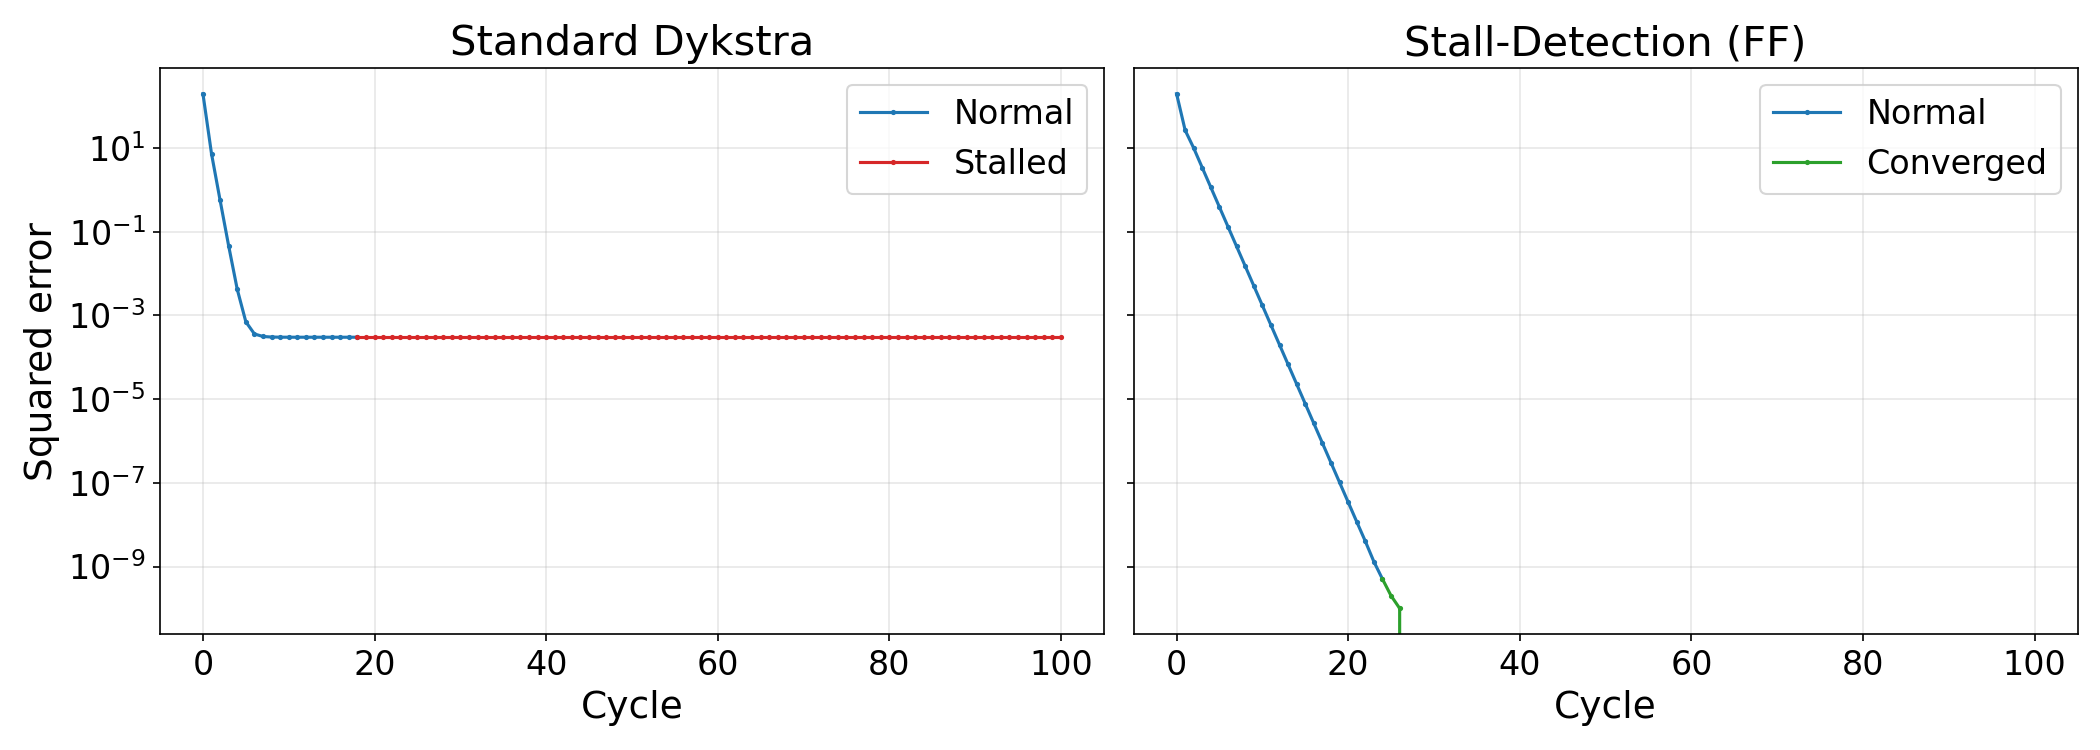
\includegraphics[width=\linewidth]{figures/benchmark_convergence_SEED=42_DIM=3_HS=6_EARLYTERMINATION.png}
        \caption{Convergence behaviour in three dimensions ($d=3$, $n=6$)}
        \label{fig:bench_3_6}
    \end{subfigure}
    
    \vspace{1em}
    
    \begin{subfigure}{\linewidth}
        \centering
        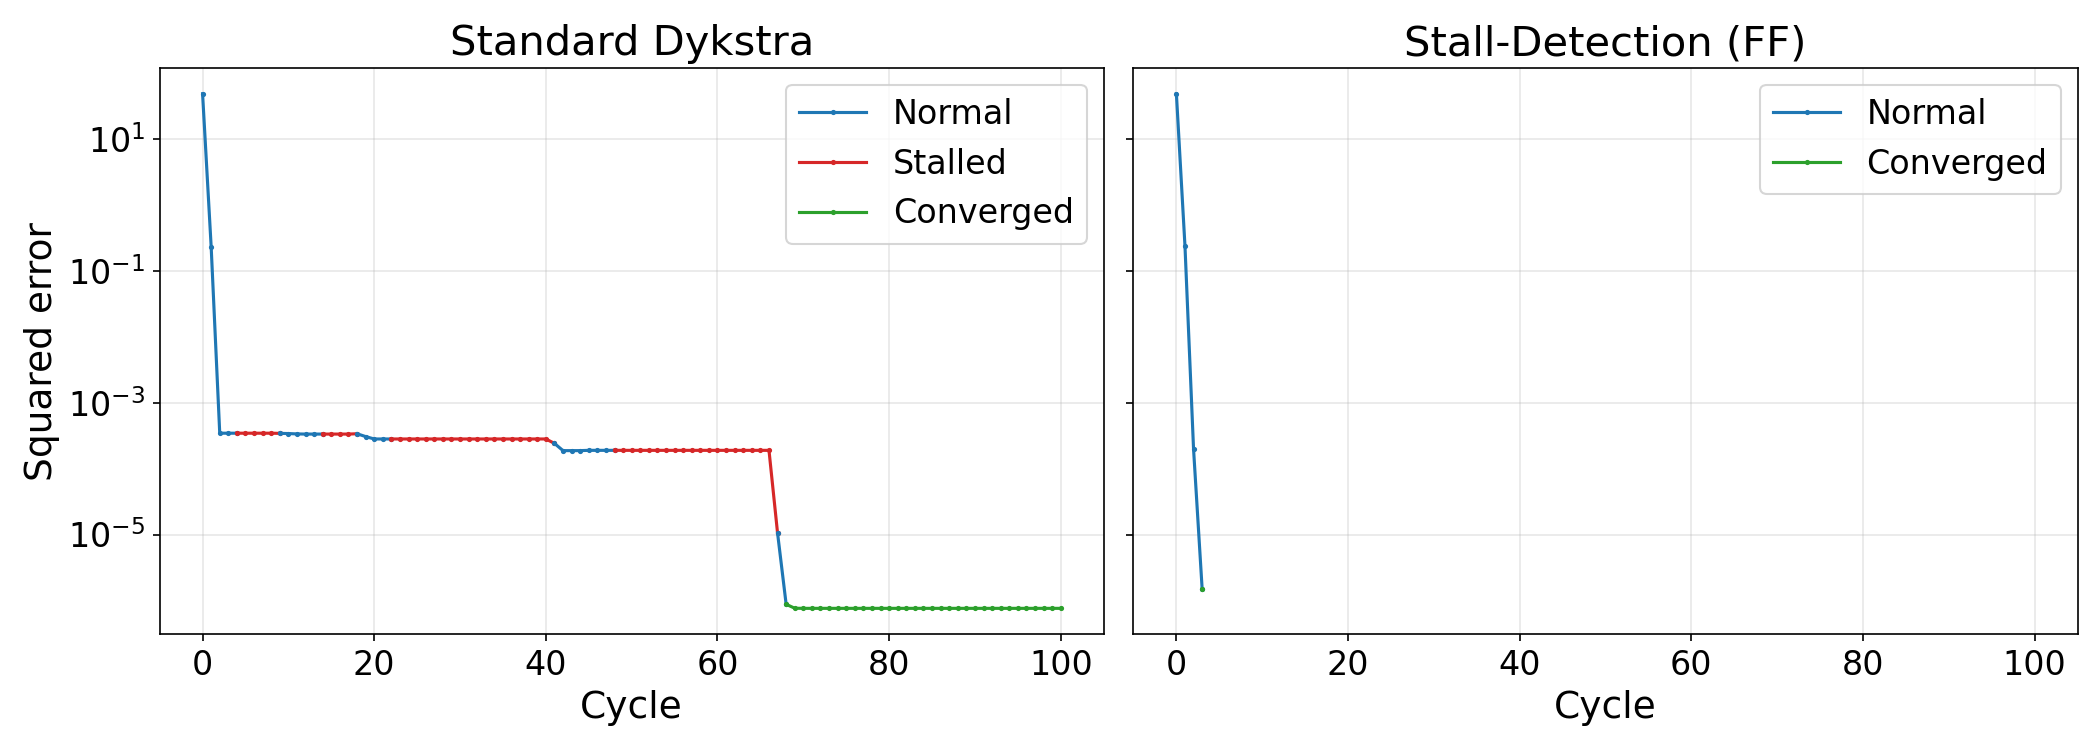
\includegraphics[width=\linewidth]{figures/benchmark_convergence_SEED=42_DIM=2_HS=20_EARLYTERMINATION.png}
        \caption{Convergence behaviour under a large number of polyhedral constraints ($d=2$, $n=20$)}
        \label{fig:bench_2_20}
    \end{subfigure}
    
    \vspace{1em}
    
    \begin{subfigure}{\linewidth}
        \centering
        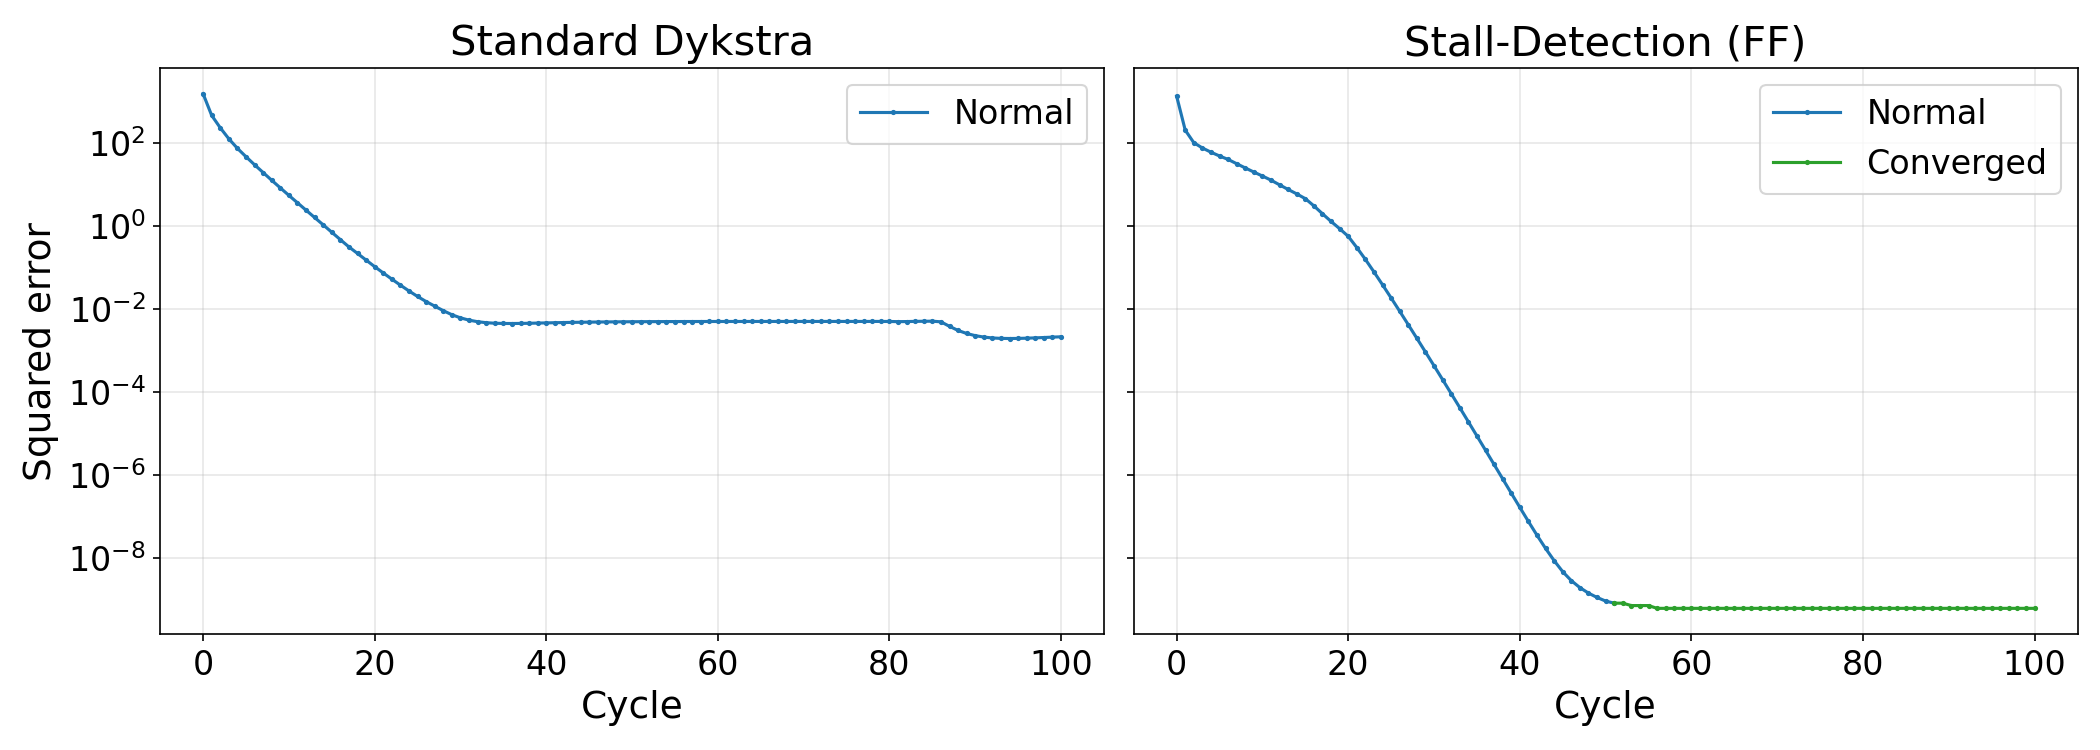
\includegraphics[width=\linewidth]{figures/benchmark_convergence_SEED=42_DIM=20_HS=50_EARLYTERMINATION.png}
        \caption{Convergence behaviour in high dimensions ($d=20$, $n=50$)}
        \label{fig:bench_20_50}
    \end{subfigure}
    
    \caption{Benchmark of Algorithm~\ref{alg:fastforward} versus Dykstra across varying geometries.}
    \label{fig:benchmark_convergence_stacked}
\end{figure}

Conversely, as seen across all three subfigures, Algorithm~\ref{alg:fastforward} eliminates the flat plateaus caused by stalling. In both low-dimensional cases (Figures~\ref{fig:bench_3_6}--\ref{fig:bench_2_20}), it breaks the initial gridlock and drives the spatial error down to high numerical precision in a handful of iterations Because the closed-form calculation proposed in Theorem~\ref{thm:nstall} relies exclusively on lightweight vector operations, the computational time overhead required to perform this detection and fast-forwarding is virtually negligible.

\begin{table}[htbp]
    \centering
    \caption{Runtime and final error across the benchmark environments.}
    \label{tab:benchmark_runtime}
    \begin{tabular}{@{}ccccc@{}}
        \toprule
        & \multicolumn{2}{c}{Standard Dykstra} & \multicolumn{2}{c}{Algorithm~\ref{alg:fastforward} (FF)} \\
        \cmidrule(lr){2-3} \cmidrule(l){4-5}
        Experiment & Time (s) & Final Error & Time (s) & Final Error \\
        \midrule
        (a) & 0.0275 & $3.01 \times 10^{-4}$ & 0.0134 & $0.00$ \\
        (b) & 0.0963 & $7.56 \times 10^{-7}$ & 0.0176 & $1.50 \times 10^{-7}$ \\
        (c) & 0.2811 & $2.15 \times 10^{-3}$ & 0.2261 & $6.00 \times 10^{-10}$ \\
        \bottomrule
    \end{tabular}
\end{table}

To quantify the direct computational advantages of bypassing stalling, the wall-clock execution time and the terminal squared spatial error $E(w^{(N_{\max})})$ were recorded for each scenario. As detailed in Table~\ref{tab:benchmark_runtime}, the fast-forward modification yields significant performance improvements across all tested geometries. In the low-dimensional configuration (a), the execution time is more than halved while driving the spatial error strictly to zero (finite-iteration convergence). Under the dense planar constraints of experiment (b), the solver achieves an 81\% reduction in runtime while maintaining comparable terminal precision. Most critically, in the high-dimensional regime (c), the modified algorithm not only reduces the overall computational runtime but also improves the final spatial accuracy by 7 orders of magnitude.